% =====================================================================
%  c06：原印刷页 47–54（PDF p.48–55）
%  §2.2.10、§2.2.11，以及两节内的三个无编号小标题
%  （Hilbert Space For Quantization Of The Flat Gauge Fields / Clock And
%   Shift Matrices / Hilbert Space For Case Of General Compact Oriented Σ2）
%  片段开头「这里 τ_IJ 是 Siegel 上半空间的一个元素」承接 c05 末尾 (2.180)，
%  仍是 §2.2.9 末尾「推广到亏格 g」小节的收尾，故此处不补任何标题。
%  公式编号 (2.181)–(2.223) 连续；本片段含图 4（figures/fig04.png，原文第 53 页）。
% =====================================================================

这里 $\tau_{IJ}$ 是 Siegel 上半空间中的一个元素。\footnote{说到底，Siegel 上半空间就是虚部正定的 $g\times g$ 对称复矩阵所构成的空间。}

一旦有了周期矩阵，就可以按 (E.65) 所给出的方式直接定义能级 $\kappa$ 的 theta 函数。作为 $\Sigma$ 上平坦规范场空间上的全纯函数，Chern-Simons 波函数是这些 theta 函数的线性组合。要把对复结构的依赖正确地纳入 Chern-Simons 波函数，就稍微麻烦一些。这会让我们进到复结构模空间上行列式线丛（determinant line bundle）的截面。物理波函数空间的一组基是

\begin{equation}
  \chi_{\beta,\kappa}(z,\tau)=\frac{\Theta_{\beta,\kappa}(z,\tau)}{\operatorname{Det}\bar\partial}
  \tag{2.181}
  \label{eq:2.181}
\end{equation}

其中 $\operatorname{Det}\bar\partial$ 是行列式线丛 $\operatorname{DET}(\bar\partial)\to\mathcal{M}_{cplx}$ 的全纯截面。

{\small\itshape ［原文标记：$\clubsuit$这一点需要多得多的解释。$\clubsuit$］}
% [原文待办标记，原文 p.47：作者自注此处解释过于简略]

具体说来：

\begin{enumerate}
  \item Hilbert 空间 $\mathcal{H}(\Sigma)$ 的复维数是 $(2\kappa)^g$。
  {\small\itshape ［原文标记：$\clubsuit$在此处补一个指向第 2.2.12 节的前向引用。$\clubsuit$］}
  % [原文待办标记，原文 p.47]
  \item 计算模群在这些函数上的作用是很直接的。
  \item 模群的作用经过 $Sp(2g;\mathbb{Z})$ 分解（factor through），而且事实上整个群 $Sp(2g;\mathbb{Z})$ 都有作用，因为 $Sp(2g;\mathbb{Z})$ 正是辛环面的辛自同构群。
  \item 高亏格的 theta 函数也有热方程的类比（原文此处引用编号缺失，印作 (??)）。
  % [原文此处 (??) 为未解析的交叉引用，原稿即如此]
\end{enumerate}

\subsubsection{环面上平坦联络的量子化：Landau 的故事} % 原文: 2.2.10 Quantization Of Flat Connections On The Torus: Landau's Story

我们还可以用一种有趣地不同的方式得到这些结果：用第 2.2.3 节所描述的、非拓扑的有质量 Chern-Simons 理论。

这里我们遵循 [26] 的做法。这一方法对于描述 AdS/CFT 对应中的 singleton（单态）自由度 [26, 8]，以及描述 M5-膜与 M 理论 C-场（C-field）的某些拓扑侧面 [45]，都非常有用。我们在这里把一般的故事作了若干简化。关于 Maxwell-Chern-Simons 理论（包括其 $p$-形式推广）完全一般的量子化，见 [20] 第 6 节。

在眼下的理论中，由于方程是线性的，运动方程解的空间（这些解不一定彼此规范等价）是一个乘积

\begin{equation}
  S=S_f\times S_{nf}
  \tag{2.182}
  \label{eq:2.182}
\end{equation}

其中 $S_f$ 是平坦解 $F=0$ 构成的空间。它们正是拓扑扇区的解。我们可以作分解 $A=A_f+A_{nf}$，其中 $A_{nf}$ 与平坦子空间正交，例如在 Hodge 度规下正交。

{\small\itshape ［原文标记：$\clubsuit$把记号从 $X$ 改成 $\Sigma_2$。本小节中的 $k$ 也要改成 $\kappa$！！！$\clubsuit$］}
% [原文待办标记，原文 p.47：作者要求统一记号，正文未改；译文照印 X 与 k]
% [Tutor Note: 这条标记是核对系数的关键线索。作者要求把本小节的 $k$ 改记为 $\kappa$（即别处 §2.2 的能级），但两处的归一化其实并不一致：把 (2.188) 的 $\omega_f=\int_X2\pi k\,\delta A\wedge\delta A$ 与第 2.2.8 小节的 (2.137) $\omega=\frac{\kappa}{\pi}da_1\wedge da_2$ 都约化到 $T^2$ 上（取 $A=a_1d\sigma^1+a_2d\sigma^2$，则 $\int_{T^2}\delta A\wedge\delta A=2\delta a_1\wedge\delta a_2$），得 $4\pi k\,\delta a_1\wedge\delta a_2=\frac{\kappa}{\pi}\delta a_1\wedge\delta a_2$，即 $k=\kappa/4\pi^2$。所以千万不要把 (2.183) 的 $2\pi k$ 直接当成 (2.136) 里的 $\kappa/2\pi$：跨小节搬用 $2\kappa$ 维数、$\frac{2\pi i}{2\kappa}$ 相位之前，先由 (2.183) 的 $2\pi k\epsilon^{ij}A_j$ 定标，否则会差出 $4\pi^2$。同理，上面条目 1 的 $(2\kappa)^g$ 也依赖于这一能级约定。]

让我们在形如 $X\times\mathbb{R}$ 的时空上把 Hamilton 形式写出来，度规为 $-dt^2+g_{ij}dx^idx^j$，定向为 $dtdx^1dx^2$。正则共轭动量（作为矢量密度）是（取 $\epsilon^{12}=+1$）：

\begin{equation}
  \Pi^i=\frac{1}{e^2}\sqrt{g}g^{ij}(\dot A_j-\partial_jA_0)+2\pi k\epsilon^{ij}A_j
  \tag{2.183}
  \label{eq:2.183}
\end{equation}

我们得到 Hamilton 密度

\begin{equation}
  \mathcal{H}=\frac{e^2}{2\sqrt{g}}g_{ij}E^iE^j+\frac{1}{2e^2}F\wedge *_2F
  \tag{2.184}
  \label{eq:2.184}
\end{equation}

其中 $*_2$ 是 $X$ 上的 Hodge 星号，并且

\begin{equation}
  E^i:=\Pi^i-2\pi k\epsilon^{ij}A_j
  \tag{2.185}
  \label{eq:2.185}
\end{equation}

（我们也会记 $E^i=\tilde\Pi^i$。）Gauss 定律是：

\begin{equation}
  \partial_i\Pi^i+2\pi k\epsilon^{ij}\partial_iA_j=0
  \tag{2.186}
  \label{eq:2.186}
\end{equation}

如果我们「在上方」（upstairs）以 $A_0=0$ 规范来表述该理论，那么相空间的坐标是 $(\Pi^i,A_i)$，辛形式为：

\begin{equation}
  \omega=\int_X\delta\Pi^i\wedge\delta A_i
  \tag{2.187}
  \label{eq:2.187}
\end{equation}

其中 $\delta$ 是无穷维相空间上的外微分。注意，当 (2.187) 被限制到平坦规范场的子空间上时，我们会得到第二类约束，而相空间就是 Chern-Simons 辛形式

\begin{equation}
  \omega_f=\int_X2\pi k\,\delta A\wedge\delta A
  \tag{2.188}
  \label{eq:2.188}
\end{equation}

它在子空间 $F=0$ 上是规范不变的，于是可以作 Hamiltonian 约化。

{\small\itshape
［原文标记：\\
*****************************************\\
这并不完全正确！正确的版本见文献 [20]\\
*****************************************］}
% [原文待办标记，原文 p.49：作者用星号框出对上面这段推导的更正声明]
% [Tutor Note: 这个星号框针对的正是 (2.187)→(2.188) 这一步。把 (2.183) 的动量代入 (2.187)，在平坦子空间上起作用的是 $2\pi k\epsilon^{ij}A_j$ 这一项（其余部分正是被第二类约束消掉的方向），得到 $\int_X2\pi k\,\epsilon^{ij}\delta A_j\wedge\delta A_i$；按 $\epsilon^{12}=+1$ 逐项展开有 $\epsilon^{ij}\delta A_j\wedge\delta A_i=-2\,\delta A_1\wedge\delta A_2$，而 (2.188) 的 $\delta A\wedge\delta A$ 展开是 $+2\,\delta A_1\wedge\delta A_2$，两者相差一个整体符号（符号由 $\epsilon^{ij}$ 的上下标位置、$dx^1dx^2$ 与 $X$ 的定向约定共同决定）。定标的最快办法仍是回到环面：把 $\omega_f$ 与第 2.2.8 小节的 (2.137) 对齐，即可同时定下符号与 $2\pi$ 因子。作者说正确版本见 [20]，指的是那里对含 $p$-形式 Maxwell-Chern-Simons 理论做了协变相空间处理。]

重新考察 $e^2\to\infty$ 极限是很有启发的。利用 (2.184)，我们看到：若限制到有限能量的场位形，则必须令 $E^i=0$。于是由 Gauss 定律必须取 $F=0$。如我们所说，限制到这个子空间会强加第二类约束，而我们正是在限制到相空间的平坦因子。

如果我们在相空间上量子化、然后再施加 Gauss 定律，则我们有波泛函 $\Psi[A_i]$，并且用辛形式 (2.187) 来量子化。因此

\begin{equation}
  \Pi^i=-i\frac{\delta}{\delta A_i}
  \tag{2.189}
  \label{eq:2.189}
\end{equation}

由于我们可以把 $A$ 分解为 $A=A_f+A_{nf}$，而 Hamiltonian 不混合这两部分，理论的 Hilbert 空间自然可以看作乘积

\begin{equation}
  H=H_f\otimes H_{nf}
  \tag{2.190}
  \label{eq:2.190}
\end{equation}

其中 $H_f$ 是平坦势的波函数空间。

Gauss 定律是：

\begin{equation}
  \Psi(A+\omega)=e^{-2\pi ik\int\omega\wedge A}\Psi(A)
  \tag{2.191}
  \label{eq:2.191}
\end{equation}

这对大规范变换同样成立。\footnote{这需要解释。恰当的数学表述是：把 $\Psi$ 看作 $X$ 上规范势空间 $\mathcal{A}(X)$ 上某个线丛的截面。然后我们提升群作用，发现只有当 $c_1(P)=0$ 时提升才存在。在这种情形下，该线丛有典范的平凡化，也有典范联络，于是波函数成为一个函数。对于更微妙的 M 理论 C-场情形，有类似的讨论 [16]。} 这里 $\omega$ 是周期为整数的闭 1-形式。注意这并不影响 $A_{nf}$ 变量。

我们将通过在实心环面上考虑该理论的欧几里得路径积分，再把该路径积分解释为沿径向的 Hamilton 演化，来确定 singleton 的 Hamiltonian。

由于我们的作用量在导数上是二阶的，在实心环面上表述路径积分时，我们应当指定边界 $X$ 上 $A_X$ 的全部分量。这与 Chern-Simons 路径积分形成对照：后者是相空间路径积分，其中我们只指定边界 $X$ 上 $A_X$ 的一个分量。

让我们考虑该理论在半径为 $\rho$ 的实心环面 $Y_\rho$ 上的欧几里得配分函数。我们假定环面的度规在渐近上表现为 $d\rho^2+\Omega^2(\rho)g_X$。路径积分定义一个态 $\Psi_{Y_\rho}(A)$，它由下式定义

\begin{equation}
  \Psi_{Y_\rho}(A)=\int\frac{dA_Y}{\operatorname{vol}\big(\mathcal{G}(Y)\big)}\,
  e^{-\int\frac{1}{2e^2}dA*dA+2\pi ik\int AdA}
  \tag{2.192}
  \label{eq:2.192}
\end{equation}

其中 $\mathcal{G}(Y)$ 是 $Y_\rho$ 上的规范群。仅凭上面关于谱的理解，我们就能明白 $\rho\to\infty$ 时的行为。

我们可以把向大 $\rho$ 的演化看作沿欧几里得时间方向的演化。大 $\rho$ 的行为投影到最低能量的态上。

\begin{equation}
  \lim_{\rho\to\infty}\Psi_{Y_\rho}(A)=e^{-\rho\,2\pi|k|e^2}\Psi_0
  \tag{2.193}
  \label{eq:2.193}
\end{equation}

其中 $\Psi_0$ 位于环面上的基态空间之中。插入 Wilson 线之类的局部算符或其他扰动，会在这个基态空间内部引起态矢量之间的跃迁。
% [Tutor Note: 指数里 $e^2$ 在分子上，即 $e^{-\rho\,2\pi|k|e^2}$，不是 $e^{-\rho\,2\pi|k|/e^2}$（放大原文 p.50 可确认）。这与「基态能量密度为 $2\pi|k|e^2$」相符：指数应为（能量密度）×（体积）$\sim\rho$，故必与 $e^2$ 成正比。若误抄成分母，则 $e^2\to\infty$ 极限会把所有态都留下，与上文「大 $\rho$ 投影到最低能态」直接矛盾——这恰是检验此处抄写是否正确的快速判据。]

\subsubsection*{平坦规范场量子化中的 Hilbert 空间} % 原文: Hilbert Space For Quantization Of The Flat Gauge Fields（原文为无编号小标题，故用 \subsubsection* 复刻）

现在考虑在 $T^2\times\mathbb{R}$ 上的量子化。我们的波函数是 $\Psi(A_f)\otimes\Psi(A_{nf})$。非平坦扇区的谱是清楚的，我们取该因子唯一的基态波函数：它就是 [15, 14] 所描述的有质量标量的各振子的谐振子基态之乘积。本小节中我们丢掉这个因子，以便专注于对 $A_f$ 的依赖。

为简单起见，我们在环面 $X=T^2$ 上工作，取 $z=\sigma^1+\tau\sigma^2$、度规 $\Omega^2|dz|^2$、$\sigma^i\sim\sigma^i+1$。我们通过假定 $A_f$ 为常数来固定小规范变换。

在复坐标 $A=A_zdz+A_{\bar z}d\bar z$ 下，我们有

\begin{equation}
  \begin{aligned}
    \tilde\Pi^{z}&=-i\left(\frac{\partial}{\partial A_z}-4\pi k\operatorname{Im}\tau\,A_{\bar z}\right)\\
    \tilde\Pi^{\bar z}&=-i\left(\frac{\partial}{\partial A_{\bar z}}+4\pi k\operatorname{Im}\tau\,A_z\right)
  \end{aligned}
  \tag{2.194}
  \label{eq:2.194}
\end{equation}

于是 Hamilton 密度为：

\begin{equation}
  \mathcal{H}=\frac{e^2}{4\operatorname{Im}\tau}
  \big(\tilde\Pi^{z}\tilde\Pi^{\bar z}+\tilde\Pi^{\bar z}\tilde\Pi^{z}\big)
  \tag{2.195}
  \label{eq:2.195}
\end{equation}

注意它们并不对易：$[\tilde\Pi^{z},\tilde\Pi^{\bar z}]=-8\pi k\operatorname{Im}\tau$。基态能量密度为 $2\pi|k|e^2$，而且是无穷重简并的，正如标准的 Landau 能级问题那样。

若 $k>0$，我们有

\begin{equation}
  \tilde\Pi^{\bar z}\Psi=0\ \Rightarrow\ \Psi=e^{-4\pi k\operatorname{Im}\tau\,A_zA_{\bar z}}\psi(A_z)
  \tag{2.196}
  \label{eq:2.196}
\end{equation}

若 $k<0$，我们有

\begin{equation}
  \tilde\Pi^{z}\Psi=0\ \Rightarrow\ \Psi=e^{4\pi k\operatorname{Im}\tau\,A_zA_{\bar z}}\psi(A_{\bar z})
  \tag{2.197}
  \label{eq:2.197}
\end{equation}

其中 $\psi$ 是全纯的。事实上，若取 $\psi=\psi_\lambda$，其中

\begin{equation}
  \psi_\lambda(x):=e^{\lambda x}
  \tag{2.198}
  \label{eq:2.198}
\end{equation}

那么波函数集合 $\{\Psi_\lambda\mid\lambda\in\mathbb{C}\}$ 是一个张成最低 Landau 能级的超完备集。
% [Tutor Note: 这两式的共轭结构极易抄错。$k>0$ 时用 $\tilde\Pi^{\bar z}\Psi=0$，得到高斯型因子 $e^{-4\pi k\operatorname{Im}\tau A_zA_{\bar z}}$ 配上全纯的 $\psi(A_z)$；$k<0$ 时方程与函数都换成「另一侧」：$\tilde\Pi^{z}\Psi=0$、因子变为 $e^{+4\pi k\operatorname{Im}\tau A_zA_{\bar z}}$、$\psi$ 变为反全纯的 $\psi(A_{\bar z})$。注意第二个指数里 $k<0$，故 $4\pi k\operatorname{Im}\tau$ 仍是负的，两种情形下 $|A|\to\infty$ 时才都衰减——这是核对上下标与符号的最省事办法（可代 $k=-1$ 验证）。]

由 (2.198) 张成的态集合是无穷维的；但当我们考虑环面上规范不变的波函数时，LLL 就变成有限维的了。我们已经通过把平坦联络取为环面上的常数，强制了小规范变换下的不变性。我们可以通过对大规范变换取平均来施加大规范变换下的不变性。给定\emph{任意}波函数 $\Psi(A)$，其平均

\begin{equation}
  \overline{\Psi}(A):=\sum_{\omega\in\mathcal{H}^1_{\mathbb{Z}}}\Psi(A+\omega)\,e^{2\pi ik\int\omega A}
  \tag{2.199}
  \label{eq:2.199}
\end{equation}

其中 $\mathcal{H}^1_{\mathbb{Z}}$ 是周期为整数的调和 1-形式，则它按 Gauss 定律 (2.191) 变换。

如果我们考虑由形如 (2.199) 的表达式所张成的 $A_z$ 的函数空间，其中取 LLL 中的函数作为试探函数，那么由于 LLL 是无穷维矢量空间，我们起初会以为由 $\overline{\Psi}(A)$ 张成的波函数矢量空间也是无穷维的。毕竟 (2.198) 中的 $\lambda$ 可以是任意复数。然而，应用 Poisson 求和公式并作一点代数运算，我们发现（这里假定 $k>0$）：

\begin{equation}
  \overline{\Psi}_\lambda
  =e^{-4\pi k\operatorname{Im}\tau\left(A_zA_{\bar z}+A_z^2\right)-\frac{\lambda^2}{16\pi k\operatorname{Im}\tau}}
  \sqrt{\frac{\tau_2}{k}}\sum_{0\le\mu<2k}
  \Theta_{-\mu,k}\big(-2i\tau_2A_z,-\bar\tau\big)\,
  \Theta_{\mu,k}\Big(\frac{-\lambda}{4\pi ik},\tau\Big)
  \tag{2.200}
  \label{eq:2.200}
\end{equation}
% [Tutor Note: 从 (2.199) 到 (2.200) 之间，作者只说「应用 Poisson 求和公式和一点代数」，省掉的正是对 $\omega\in\mathcal{H}^1_{\mathbb{Z}}\cong\mathbb{Z}^2$ 作 Poisson 重求和：重求和把 $\Psi(A+\omega)$ 在格上的和变成对偶格上的和，即 $\mu$ 的有限和（$0\le\mu<2k$），于是无穷维的 LLL 被压成 $2k$ 维。核对时注意两个 theta 函数的模参数不是同一个：第一个用 $-\bar\tau$、第二个用 $\tau$；宗量分别是 $-2i\tau_2A_z$ 与 $-\lambda/(4\pi ik)$。若不放心，可用 (2.201) 的归一化因子 $k^{3/4}/\bar\eta$ 反推 (2.200) 的指数（$\bar\eta$ 说明这里用的是反全纯的模参数），比重新做一遍 Poisson 求和快得多，详见 [17, 26]。]

这个公式表明，作为 $A_z$ 的函数，我们只得到一个有限维空间。事实上可以证明（见 [17, 26]），平坦规范场扇区的一组归一化波函数基是：

\begin{equation}
  \psi_\mu=\frac{k^{3/4}}{\bar\eta}\,
  e^{-4\pi k\operatorname{Im}\tau\left(A_zA_{\bar z}+A_z^2\right)}
  \Theta_{-\mu,k}\big(-2i\tau_2A_z,-\bar\tau\big)
  \tag{2.201}
  \label{eq:2.201}
\end{equation}

\subsubsection{环面上平坦联络的量子化：Heisenberg 的故事} % 原文: 2.2.11 Quantization Of Flat Connections On The Torus: Heisenberg's Story

万一你对刚才得到的结果还不够放心，让我们从 Heisenberg 群的观点来看一看。

经典地，和乐由 $U_i=\exp[ia_i]$ 描述。量子地，我们得到算符：

\begin{equation}
  \widehat{U}_i=\exp[i\hat a_i]
  \tag{2.202}
  \label{eq:2.202}
\end{equation}

由对易子 \eqref{eq:2.143} 可得

\begin{equation}
  \widehat{U}_1\widehat{U}_2=e^{\frac{2\pi i}{2\kappa}}\widehat{U}_2\widehat{U}_1
  \tag{2.203}
  \label{eq:2.203}
\end{equation}

特别地，

\begin{equation}
  \widehat{U}_1\widehat{U}_2\widehat{U}_1^{-1}=e^{\frac{2\pi i}{2\kappa}}\widehat{U}_2
  \tag{2.204}
  \label{eq:2.204}
\end{equation}

这意味着 $U_1$ 把 $a_2$ 平移 $2\pi/2\kappa$，类似地 $U_2$ 平移 $a_1$。因此我们还有如下关系：

\begin{equation}
  \widehat{U}_1^{2\kappa}=\widehat{U}_2^{2\kappa}=1
  \tag{2.205}
  \label{eq:2.205}
\end{equation}

(2.204) 与 (2.205) 定义了一个有限非阿贝尔群，称为有限 Heisenberg 群。一般地，对任意整数 $N$，存在一个阶为 $N^3$ 的 Heisenberg 群。它处于一个（非分裂的）正合列中

\begin{equation}
  1\to\mathbb{Z}_N\to\mathrm{Heis}_N\to\mathbb{Z}_N\oplus\mathbb{Z}_N\to 0
  \tag{2.206}
  \label{eq:2.206}
\end{equation}

它是量子力学中通常的 Heisenberg 关系的有限群类比。

有一个标准定理，即 Stone-von Neumann 定理，它说：在同构意义下，Heisenberg 群的酉不可约表示是唯一的，其中 $U(1)$ 中的标量就简单地作用为乘以该标量。对所有 Heisenberg 群这都是对的，因此 $\mathrm{Heis}_N$ 有唯一的不可约表示。
% [Tutor Note: 作者这句话省掉了 SvN 定理的两个前提：(i) 表示须以给定的中心特征（central character）$\chi:U(1)\to U(1)$ 作用，定理说的唯一性是「在该中心特征给定之后」；(ii) 群律里的 2-上闭链（即 (2.203) 的相位）须与给定的辛形式/相交形式相容。证明只是 Schur 引理加维数计数：不可约表示的维数平方等于中心 $\mathbb{Z}_N$ 的大小 $N^2$，故维数必为 $N$；有限 Heisenberg 群的这一结论与连续情形（Stone-von Neumann 唯一性定理）是同一件事的两种版本。译者取舍：「representation」在本段既指 $U(1)$ 的电荷 $n$ 表示（纤维上的作用），又指 Heisenberg 群在 Hilbert 空间上的表示，二者都译作「表示」；缩写 SvN 保留（后文 (2.223) 处作者自己就写 SvN）。]

\subsubsection*{钟矩阵与移位矩阵} % 原文: Clock And Shift Matrices（原文为无编号小标题，故用 \subsubsection* 复刻）

呈现 Heisenberg 群 $\mathrm{Heis}_N$ 的 Stone-von Neumann 表示的一种标准方式，是通过 $N\times N$ 的「钟」（clock）矩阵与「移位」（shift）矩阵 $P$ 与 $Q$。为定义它们，引入一个 $N$ 次单位根，比如 $\omega=\exp[2\pi i/N]$。于是

\begin{equation}
  P_{i,j}=\delta_{i=j+1\operatorname{mod}N}
  \tag{2.207}
  \label{eq:2.207}
\end{equation}

\begin{equation}
  Q_{i,j}=\delta_{i,j}\omega^{j}
  \tag{2.208}
  \label{eq:2.208}
\end{equation}

注意 $P^N=Q^N=1$，且没有更小的幂等于 1。进而注意\footnote{检查这一点——从而检查你的约定是否在掌控之中——最快的办法是计算 $QPQ^{-1}$，因为 $(Q^{-1}PQ)_{ij}=Q_{ii}P_{ij}(Q_{jj})^{-1}=\omega P_{ij}$。}

\begin{equation}
  QP=\omega PQ
  \tag{2.209}
  \label{eq:2.209}
\end{equation}

当 $N=4$ 时，这两个矩阵形如

\begin{equation}
  P=
  \begin{pmatrix}
    0&0&0&1\\
    1&0&0&0\\
    0&1&0&1\\
    0&0&1&0
  \end{pmatrix}
  \qquad\qquad
  Q=
  \begin{pmatrix}
    \omega&0&0&0\\
    0&\omega^2&0&0\\
    0&0&\omega^3&0\\
    0&0&0&1
  \end{pmatrix}
  \tag{2.210}
  \label{eq:2.210}
\end{equation}

其中 $\omega=e^{2\pi i/4}$。由 $P,Q$ 生成的矩阵群是 $GL(N,\mathbb{C})$ 的一个有限子群，同构于一个有限 Heisenberg 群。在量子化一个在群 $U(1)$ 上运动、但被限制在 $N$ 阶循环子群内的量子粒子时，人们自然会遇到它们。
% [Tutor Note: 印出的 $P$ 第三行「$0\ 1\ 0\ 1$」含两个 1，不是置换矩阵，此时 $P^N=1$（更不必说「没有更小的幂等于 1」）并不成立：由 $Pe_4=e_1+e_3$ 可见 $P$ 会把某些向量越打越长。按 (2.207) 的定义 $P_{i,j}=\delta_{i=j+1\bmod N}$（$j=1,\dots,N$），$N=4$ 时应为 $(0\,0\,0\,1),(1\,0\,0\,0),(0\,1\,0\,0),(0\,0\,1\,0)$。旁证：$Q$ 的印出值 $\mathrm{diag}(\omega,\omega^2,\omega^3,1)$ 与 (2.208) 的 $Q_{i,j}=\delta_{i,j}\omega^j$ 完全一致，说明索引确从 $j=1$ 取到 $N$。此处照印未改，使用时请以定义 (2.207) 为准。]

{\small\itshape ［原文标记：$\clubsuit$关于这一点能给更多细节吗？$\clubsuit$］}
% [原文待办标记，原文 p.52：作者自注此处（U(1) 上粒子的量子化）解释不足]

\textbf{评注}：由 $P,Q$ 生成的算符代数是完整的矩阵代数 $\mathrm{Mat}_{N\times N}(\mathbb{C})$。也就是说，态空间上的任意线性变换都可以写成乘积 $P^mQ^n$ 的线性组合。

{\small\itshape ［原文标记：$\clubsuit$也许该多说说如何用有限 Fourier 变换来做这件事。$\clubsuit$］}
% [原文待办标记，原文 p.52]

\subsubsection*{一般紧定向曲面 $\Sigma_2$ 情形的 Hilbert 空间} % 原文: Hilbert Space For Case Of General Compact Oriented Σ2（原文为无编号小标题，故用 \subsubsection* 复刻）

{\small\itshape ［原文标记：$\clubsuit$为了与前面一致、并区分路径积分中插入的线缺陷与 Hilbert 空间上的算符，或许该给这些算符 $\widehat{W}(n,\gamma)$ 都加个帽子。$\clubsuit$］}
% [原文待办标记，原文 p.53：正文中确实混用了带帽与不带帽的写法]

我们可以轻而易举地把上面的讨论推广到一般紧定向曲面 $\Sigma_2$：若 $\gamma\subset\Sigma_2$ 是一条定向闭圈，$V_n$ 是 $U(1)$ 的电荷 $n$ 表示，$n\in\mathbb{Z}$，则可以构造 Wilson 线算符 $W(n,\gamma)=\exp[in\oint_\gamma A]$，见 \eqref{eq:2.61}。由于规范场是平坦的，它（在没有其他算符的情况下）只依赖于 $\gamma$ 的\underline{同调类}。特别地，相当平凡地

\begin{equation}
  \exp\Big[in\oint_\gamma A\Big]=\exp\Big[i\oint_{n\gamma}A\Big]
  \tag{2.211}
  \label{eq:2.211}
\end{equation}

有相应的量子算符。我们可以把它们写成：

\begin{equation}
  \widehat{W}(n,\gamma):=\exp\Big[in\oint_\gamma\widehat{A}\Big]
  \tag{2.212}
  \label{eq:2.212}
\end{equation}

同样，这个算符只依赖于乘积，所以我们可以简化，只用一个单变量 $\gamma\in H_1(\Sigma_2;\mathbb{Z})$ 的算符值函数 $\widehat{W}(\gamma)$ 来工作。

这些算符依赖于 $\gamma$ 的定向，并且我们有

\begin{equation}
  \widehat{W}(-\gamma)=\widehat{W}(\gamma)^{\dagger}=\widehat{W}(\gamma)^{-1}
  \tag{2.213}
  \label{eq:2.213}
\end{equation}

那么 (2.204) 的推广要用 Baker-Campbell-Hausdorff 公式以及 (2.87) 的对易子。结果是

\begin{equation}
  \widehat{W}(\gamma_1)\widehat{W}(\gamma_2)
  =e^{\frac{2\pi i}{2\kappa}I(\gamma_1,\gamma_2)}
  \widehat{W}(\gamma_2)\widehat{W}(\gamma_1)
  \tag{2.214}
  \label{eq:2.214}
\end{equation}

其中

\begin{equation}
  I(\gamma_1,\gamma_2)=\sum_{p\in\gamma_1\cap\gamma_2}\iota_p(\gamma_1,\gamma_2)
  \tag{2.215}
  \label{eq:2.215}
\end{equation}

是 $\gamma_1$ 与 $\gamma_2$ 的定向相交数。

\begin{figure}[htbp]
  \centering
  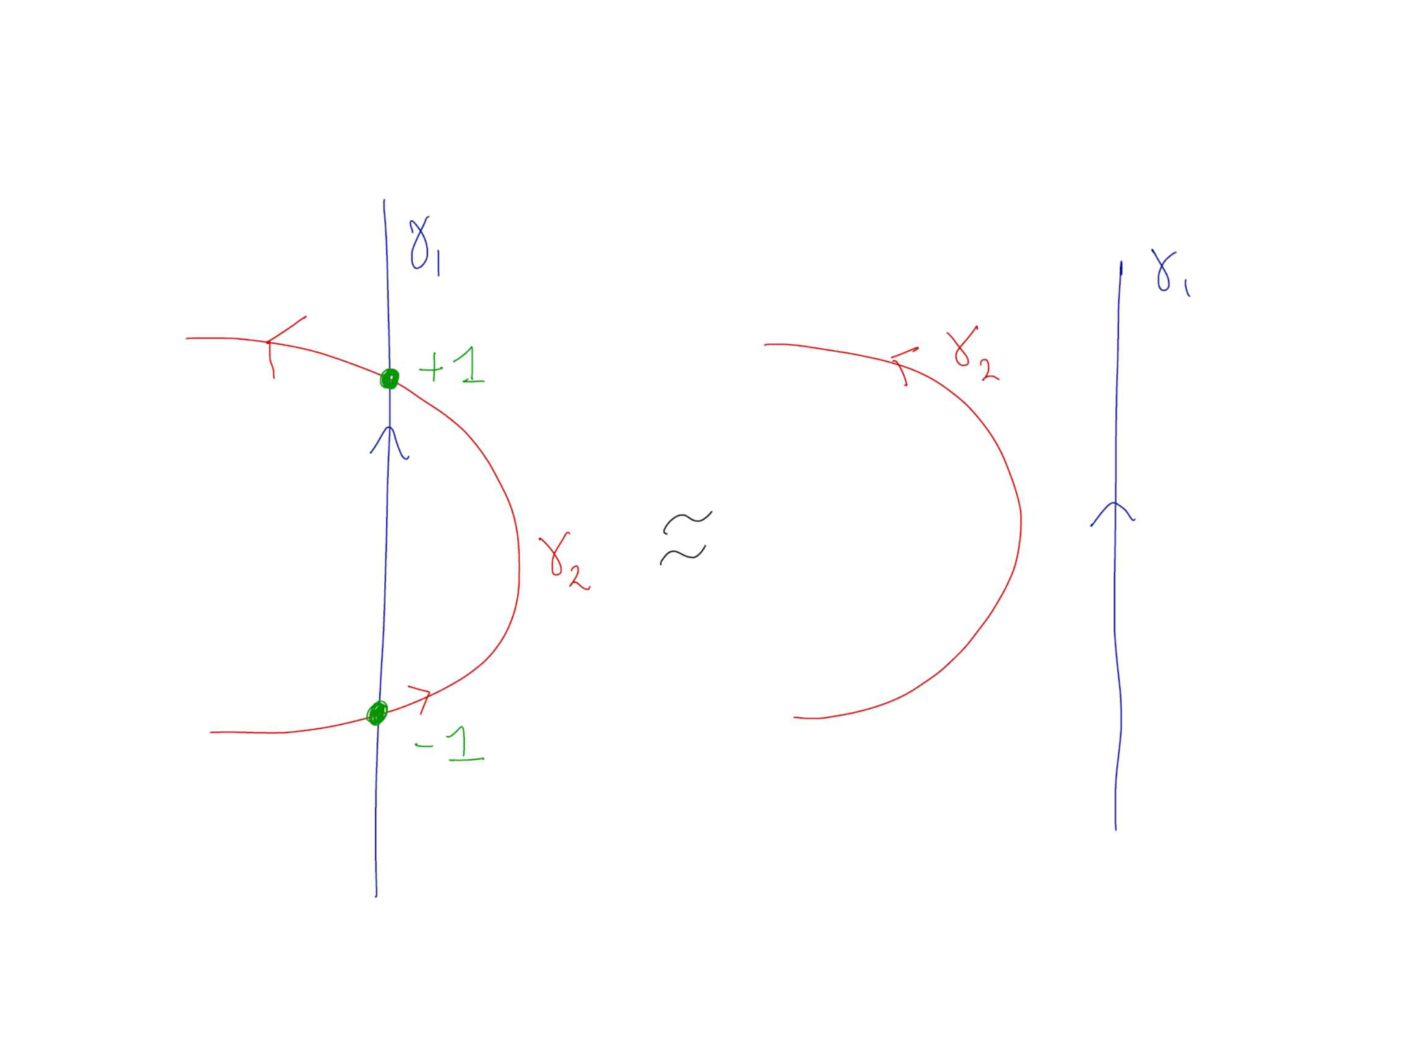
\includegraphics[width=0.78\textwidth]{figures/fig04.png}
  \caption{由于相交数是有符号的求和，其符号由定向决定，总的相交数在形变下不变，此处以一个简单情形加以说明。对横截相交的曲线求定向交点之和，给出一个只依赖于这些曲线的同调类的不变量。（原文 Fig.~4，第 53 页）}
  \label{fig:4}
\end{figure}
% [原文图注的英文原句有笔误：「with the sign determined by the orientation to total intersection number is invariant」应为「...by the orientation, the total intersection number is invariant」；此处按文意译出，未增删内容。]

为定义定向相交数，我们假定 $\gamma_1$ 与 $\gamma_2$ 处于一般位置（general position），从而交点只有有限多个，且都是横截的。于是，在每个交点 $p\in\gamma_1\cap\gamma_2$ 处，切矢量 $\{\dot\gamma_1(p),\dot\gamma_2(p)\}$ 构成 $T_p\Sigma_2$ 的一个有序基。因此它们定义了矢量空间 $T_p\Sigma_2$ 的一个定向 $o_{12}(p)$。另一方面，我们假定 $\Sigma_2$ 带有一个定向 $o_\Sigma$，于是可以比较 $o_{12}(p)$ 与 $o_\Sigma(p)$。我们可以定义

\begin{equation}
  \iota_p(\gamma_1,\gamma_2):=
  \begin{cases}
    +1 & o_{12}(p)=o_{\Sigma_2}(p)\\
    -1 & o_{12}(p)\ne o_{\Sigma_2}(p)
  \end{cases}
  \tag{2.216}
  \label{eq:2.216}
\end{equation}

然后可以证明，(2.215) 事实上只依赖于 $\gamma_1$ 与 $\gamma_2$ 的同调类。基本想法如图~\ref{fig:4} 所示。定向相交数使阿贝尔群 $H_1(\Sigma_2;\mathbb{Z})$ 成为一个辛格（symplectic lattice），因此我们常把相交记作 $\langle\gamma_1,\gamma_2\rangle:=I(\gamma_1,\gamma_2)$。

{\small\itshape ［原文标记：$\clubsuit$在此处作解释或引用文献。$\clubsuit$］}
% [原文待办标记，原文 p.54：边注，位置在上段「使…成为辛格」处]

由于算符 $\widehat{W}(\gamma)$ 是酉的，它们生成的算符代数就是所谓的非交换环面代数（noncommutative torus algebra）。关于一般性的评述见下文。

{\small\itshape ［原文标记：$\clubsuit$我们是否该论证一下它是一个 $C^*$ 代数或 $W^*$ 代数？$\clubsuit$］}
% [原文待办标记，原文 p.55：边注，插在「见下文。One / can show」之间]

可以证明这些算符满足如下关系：

\begin{equation}
  \widehat{W}(\gamma_1)\widehat{W}(\gamma_2)
  =e^{\frac{\pi i}{2\kappa}I(\gamma_1,\gamma_2)}
  \widehat{W}(\gamma_1+\gamma_2)
  \tag{2.217}
  \label{eq:2.217}
\end{equation}
% [Tutor Note: (2.214) 与 (2.217) 的指数相差一个因子 2：$\frac{2\pi i}{2\kappa}I$ 对 $\frac{\pi i}{2\kappa}I$。这个 $1/2$ 不是笔误，也不是靠 BCH 直接得到的，而是把「两算符之积」改写为「单个算符乘中心相位」时的必然后果：由 (2.217) 按两种次序写 $\widehat{W}(\gamma_1+\gamma_2)$，得 $e^{-\frac{\pi i}{2\kappa}I(\gamma_1,\gamma_2)}\widehat{W}(\gamma_1)\widehat{W}(\gamma_2)=e^{+\frac{\pi i}{2\kappa}I(\gamma_1,\gamma_2)}\widehat{W}(\gamma_2)\widehat{W}(\gamma_1)$（用了 $I(\gamma_2,\gamma_1)=-I(\gamma_1,\gamma_2)$），两式相比即回到 (2.214)，指数里的 2 正是 (2.217) 的 $1/2$ 的两倍。也正因如此，作者才说须先取 $H_1$ 的一组基、再适当定义 $\widehat{W}(\gamma)$，即选定截面的平凡化。检验办法：把 (2.223) 的显式表示代入，对 $\gamma\in L_b$ 由 (2.217) 应得相位 $e^{2\pi i\langle\gamma,\gamma_0\rangle/2\kappa}$。]

（这并不能由 BCH 公式直接推出。不过，可以取 $H_1(\Sigma_2;\mathbb{Z})$ 的一组基，并以适当方式对一般的 $\gamma$ 定义 $\widehat{W}(\gamma)$，使得 (2.217) 成立。）

现在，满足 (2.214) 的酉算符代数的中心由 $W(n,\gamma)^{2\kappa}$ 生成，所以我们可以把这些元素取为 1。确实，我们在环面的情形已经看到，必须把它们取为 1。因此 $W(n,\gamma)$ 只依赖于 $n\sim n+2\kappa$，并且我们有乘积法则：

\begin{equation}
  \widehat{W}(n_1,\gamma)\widehat{W}(n_2,\gamma)=\widehat{W}(n_1+n_2,\gamma)
  \tag{2.218}
  \label{eq:2.218}
\end{equation}

其中加法是模 $2\kappa$ 的。

Heisenberg 群的一般理论再一次变得非常有用。我们有一个非分裂的中心扩张

\begin{equation}
  1\to\mathbb{Z}/2\kappa\mathbb{Z}\to
  \mathrm{Heis}\big(H_1(\Sigma_2;\mathbb{Z}/2\kappa\mathbb{Z})\big)\to
  H_1(\Sigma_2;\mathbb{Z}/2\kappa\mathbb{Z})\to 1
  \tag{2.219}
  \label{eq:2.219}
\end{equation}

其中我们把中心群 $\mathbb{Z}/2\kappa\mathbb{Z}\subset U(1)$ 看作 $(2\kappa)$ 次单位根构成的群。Stone-von Neumann 表示在同构意义下是唯一的，而只要选取一个极大的拉格朗日分解，就可以把它显式给出

\begin{equation}
  H_1(\Sigma_2;\mathbb{Z}/2\kappa\mathbb{Z})\cong L_1\oplus L_2
  \tag{2.220}
  \label{eq:2.220}
\end{equation}

这样的拉格朗日子空间相当于如图~\ref{fig:3} 那样区分 $a$-圈与 $b$-圈。于是我们记 $L_1=L_a$、$L_2=L_b$：

\begin{equation}
  H_1(\Sigma_2;\mathbb{Z}/2\kappa\mathbb{Z})\cong L_a\oplus L_b
  \tag{2.221}
  \label{eq:2.221}
\end{equation}

为给出显式的 SvN 表示，我们考虑，比如说，拉格朗日子群 $L_a$ 上的 $L^2$ 函数。作为阿贝尔群，$L_a$（非典范地）是

\begin{equation}
  L_a\cong\mathbb{Z}_{2\kappa}\oplus\cdots\oplus\mathbb{Z}_{2\kappa}
  \tag{2.222}
  \label{eq:2.222}
\end{equation}

共有 $g$ 个直和项。因此这个有限群上的 $L^2$ 函数空间是 $(2\kappa)^g$ 维的。该表示由下述方式确定：使用规则 (2.217)，然后给出 $W(\gamma)$ 在 $\gamma$ 限制到两个拉格朗日子空间时的作用：

\begin{equation}
  \begin{aligned}
    \widehat{W}(\gamma)\Psi(\gamma_0)&=\Psi(\gamma_0+\gamma) && \gamma\in L_a\\
    \widehat{W}(\gamma)\Psi(\gamma_0)&=e^{2\pi i\frac{\langle\gamma,\gamma_0\rangle}{2\kappa}}\Psi(\gamma_0)
    && \gamma\in L_b
  \end{aligned}
  \tag{2.223}
  \label{eq:2.223}
\end{equation}

{\small\itshape ［原文标记：$\clubsuit$还有，应该加一个附录，讲 Heisenberg 群的一般 SvN 表示。$\clubsuit$］}
% [原文待办标记，原文 p.54]
